%!TEX root = ../../thesis.tex
\chapter{Influenza Evolution}
\label{ch:influenza}

In this chapter we analyze influenza.
Influenza is useful to examine because there is a lot of data.

\section{Influenza Virus}

Influenza is a single-stranded RNA virus that is naturally found in avian populations.
Each viral genome has eight genetic segments.

\section{Reassortment}

The evolution of influenza is punctuated by frequent reassortment.
To characterize influenza evolution, we computed the persistent homology of four influenza datasets from avian, swine, and human hosts, each numbering as many as 1,000 genomic sequences.
When applied to a single segment of the virus unaffected by reassortment, higher-dimensional homology groups vanish (Fig. 2).
Alignments of single segments are therefore suitable for phylogenetic analysis.
In settings of vertical evolution, we can directly transform a filtration of 0-D simplicial complexes into an equivalent distance-based dendrogram.
 Fig. 2A represents the zero-dimensional topology of the hemagglutinin segment of avian influenza viruses. 
 The zero-dimensional generators at higher genetic distances indicate the major clusters, coinciding with the antigenic subtypes H1-H16.
 From the bar sizes of the barcode plot, we can create a dendrogram that recapitulates classic phylogenetic analyses57,58 (Fig. 2B).
 Only when segments are concatenated does persistent homology indicate that reassortment precludes phylogenetic analysis (Fig. 2C).
 These results show that persistent homology can detect pervasive reassortment in influenza.
 Estimating ICR from one-dimensional homology provides a lower-bound on reassortment rate in influenza.
 We calculate an ICR of <1 event per year for classic H1N1 swine and H3N2 human influenza viruses, supported by previous phylogenetic estimates59,60.
 In contrast, we calculate a high reassortment rate of 22.16 events per year for avian influenza A.
This difference could be explained by the high diversity and frequent co-infection of avian viruses and correlates with the high proportion of potential avian reassortants reported in previous studies61,62.

\section{Multiscale Flu Reassortment}

\begin{figure}
\begin{center}
\centerline{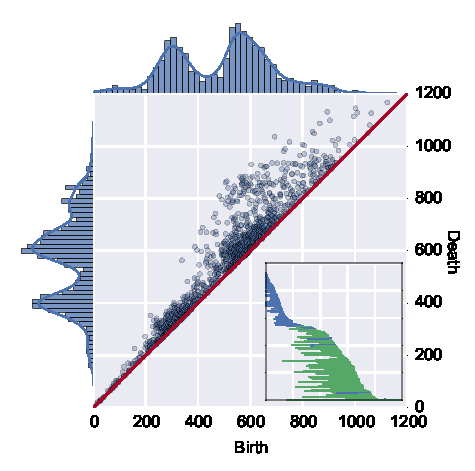
\includegraphics[width=\columnwidth]{./fig/flu_scatterplot.pdf}}
\caption[$H_1$ persistence diagram computed from an avian influenza dataset.]{The $H_1$ persistence diagram computed from an avian influenza dataset. On the top and left are plotted the marginal distributions of birth and death times, along with a density estimate for each distribution. The bimodality indicates two scales of topological structure. Inset: The barcode diagram for a subset of this data. Blue bars have representative cycles involving only one subtype, green bars have cycles involving multiple subtypes.}
\label{fig:flu_scatterplot}
\end{center}
\end{figure}

To test our model on biological data, we considered reassortment in avian influenza virus.
Influenza is a single-stranded RNA virus that is naturally found in avian populations.
Each viral genome has eight genetic segments.
Subtypes are defined by two segments, hemagglutinin (HA) and neuraminidase (NA), e.g. H1N1 and H3N2.
When a host cell is coinfected with two different viral strains, reassortment of these segments can occur, such that viral offspring is a genetic mixture of the two parental strains.
Reassortment is of substantial medical interest, and has been connected with the outbreak of influenza epidemics.

We computed persistent homology on an aligned dataset of 3,105 avian influenza sequences across the seven major HA subtypes.
The persistence diagram is shown in Figure \ref{fig:flu_scatterplot}, along with density estimates for the birth and death distributions.
Both birth and death times appear strongly bimodal, unlike in the coalescent simulations, which were strictly unimodal.
This suggests two distinct scales of topological structure.
Using the representative cycles output by Dionysus on a subset of this data, we classified features as intrasubtype (involving one HA subtype) and intersubtype (involving multiple HA subtypes).
The $H_1$ barcode diagram for this data is shown in the Figure \ref{fig:flu_scatterplot} inset.
Intrasubtype features, in blue, occur at an earlier filtration scale than intersubtype features, in green.
The multiscale topological approach of persistent homology can distinguish biological events occuring at different genetic scales.

We isolated the two peaks and estimated two recombination rates: an intrasubtype $\rho_{1}=9.68$, and an intersubtype $\rho_{2}=21.43$.
We conclude that intersubtype recombination occurs at a rate over twice that of intrasubtype recombination, however a genetic barrier exists that maintains distinct subtype populations.
The nature of this barrier warrants further study.
This illustrates a real world example in which multiscale topological structure can be captured by persistent homology and given biological interpretation.

\section{Prediction of Host Specific Residues}

In this section, we describe work in prediction of host specific residues using machine learning approaches.
Host specific residues are important for viral surveillance in order to predict possible outbreaks.
We describe here two methods and include preliminary validation from our collaborator in Wisconsin.